\documentclass[12pt]{article}
\usepackage[margin=2.5cm]{geometry}
\usepackage{titling}
\usepackage{enumerate}
\usepackage{graphicx}
\usepackage{mdframed}
\usepackage{listings}
\usepackage{xcolor}
\usepackage{hyperref}
\usepackage[utf]{kotex}

\definecolor{codegreen}{rgb}{0,0.6,0}
\definecolor{codegray}{rgb}{0.5,0.5,0.5}
\definecolor{codepurple}{rgb}{0.58,0,0.82}
\definecolor{backcolour}{rgb}{0.95,0.95,0.92}

\lstdefinestyle{mystyle}{
    backgroundcolor=\color{backcolour},
    commentstyle=\color{codegreen},
    keywordstyle=\color{magenta},
    numberstyle=\tiny\color{codegray},
    stringstyle=\color{codepurple},
    basicstyle=\ttfamily\footnotesize,
    breakatwhitespace=false,
    breaklines=true,
    captionpos=b,
    keepspaces=true,
    numbers=left,
    numbersep=5pt,
    showspaces=false,
    showstringspaces=false,
    showtabs=false,
    tabsize=1
}

\lstset{style=mystyle}

\predate{}
\postdate{}

\begin{document}
\title{Lab 4: Abstract Data Type Solution}
\date{}
\maketitle

\section*{4) Additional Tasks}
\subsection*{Graphing your results}
\begin{enumerate}[1.]
    \item Implement \textit{time\_queue\_lists}, a modified version of your timing
    experiment function that returns a tuple containing three lists:

    \begin{itemize}
        \item A list of queue sizes it tried
        \item A list of the corresponding times to run enqueue for each queue size
        \item A list of the corresponding times to run dequeue for each queue size
    \end{itemize}

    \bigskip

    Note that each of your lists should have the same length.

    \bigskip

    \begin{mdframed}
        \begin{lstlisting}[language=Python,caption={task\_4\_q1\_part\_1\_solution.py},captionpos=b]
        ...
        def time_queue_lists() -> Tuple[List[int], List[float], List[float]]:
            """Run timing experiments for Queue.enqueue and Queue.dequeue.

            Return lists storing the results of the experiments.  See the lab
            handout for further details.
            """
            queue_sizes = [10000, 20000, 40000, 80000, 160000]
            enqueue_time_list = []
            dequeue_time_list = []

            trials = 200

            for queue_size in queue_sizes:
                queues = _setup_queues(queue_size, trials)

                time = 0
                for queue in queues:
                    time += timeit('queue.enqueue(1)', number=1, globals=locals())

                print(f'enqueue: Queue size {queue_size:>7}, time {time}')
                enqueue_time_list.append(time)

            for queue_size in queue_sizes:
                queues = _setup_queues(queue_size, trials)

                time = 0
                for queue in queues:
                    time += timeit('queue.dequeue()', number=1, globals=locals())

                print(f'dequeue: Queue size {queue_size:>7}, time {time}')
                dequeue_time_list.append(time)

            return (queue_sizes, enqueue_time_list, dequeue_time_list)

        ...
        \end{lstlisting}
    \end{mdframed}

    \item To actually plot the data, we’ll use the Python library \textit{matplotlib},
    which is an extremely powerful and popular library for plotting all sorts of
    data.

    \bigskip

    If you’re on a Teaching Lab machine, you already have this library installed.

    \bigskip

    If you’re on your own machine, you should have already installed this library
    by following the CSC148 Software Guide. (Look for the section on installing
    Python libraries.)

    \bigskip

    Add the statement \textit{import matplotlib.pyplot as plt} to the top of \textit{timequeue.py},
    and make sure you can still run your file without error.

    \bigskip

    \begin{mdframed}

    \begin{lstlisting}[language=Python,caption={task\_4\_q1\_part\_2\_solution.py},captionpos=b]
    ...
    import matplotlib.pyplot as plt
    ...
    \end{lstlisting}

    \bigskip

    \underline{\textbf{Note:}}

    \begin{itemize}
        \item
        If \textit{matplotlib} is missing, install by typing \textit{pip3 install matplotlib}
        in terminal or windows command line.
    \end{itemize}

    \end{mdframed}

    \item To get a basic 2-D plot of your timing data, work your way through the
    first part of \href{https://matplotlib.org/users/pyplot_tutorial.html}{this guide} (Links to an external site.). (Ignore all of the
    references to “numpy”, which is another Python library we aren’t using in this
    course. Also ignore the other sections after the first one; the whole tutorial
    is pretty long!)

    \bigskip

    You can use an x-axis range of 0-200000 and a y-axis range of 0-0.02 (feel
    free to adjust the y-axis depending on how long the experiments take to run
    on your computer).

    \bigskip

    \begin{mdframed}

    \begin{lstlisting}[language=Python,caption={task\_4\_q1\_part\_3\_solution.py},captionpos=b]
    if __name__ == '__main__':
        ...
        plt.plot(queue_sizes, enqueue_time_list, 'ro')
        plt.plot(queue_sizes, dequeue_time_list, 'bo')
        plt.xlim([0,200000])
        plt.ylim([0,0.02])
        plt.xlabel('Queue Size')
        plt.ylabel('Time (Seconds)')
        plt.show()
    \end{lstlisting}

    \begin{center}
    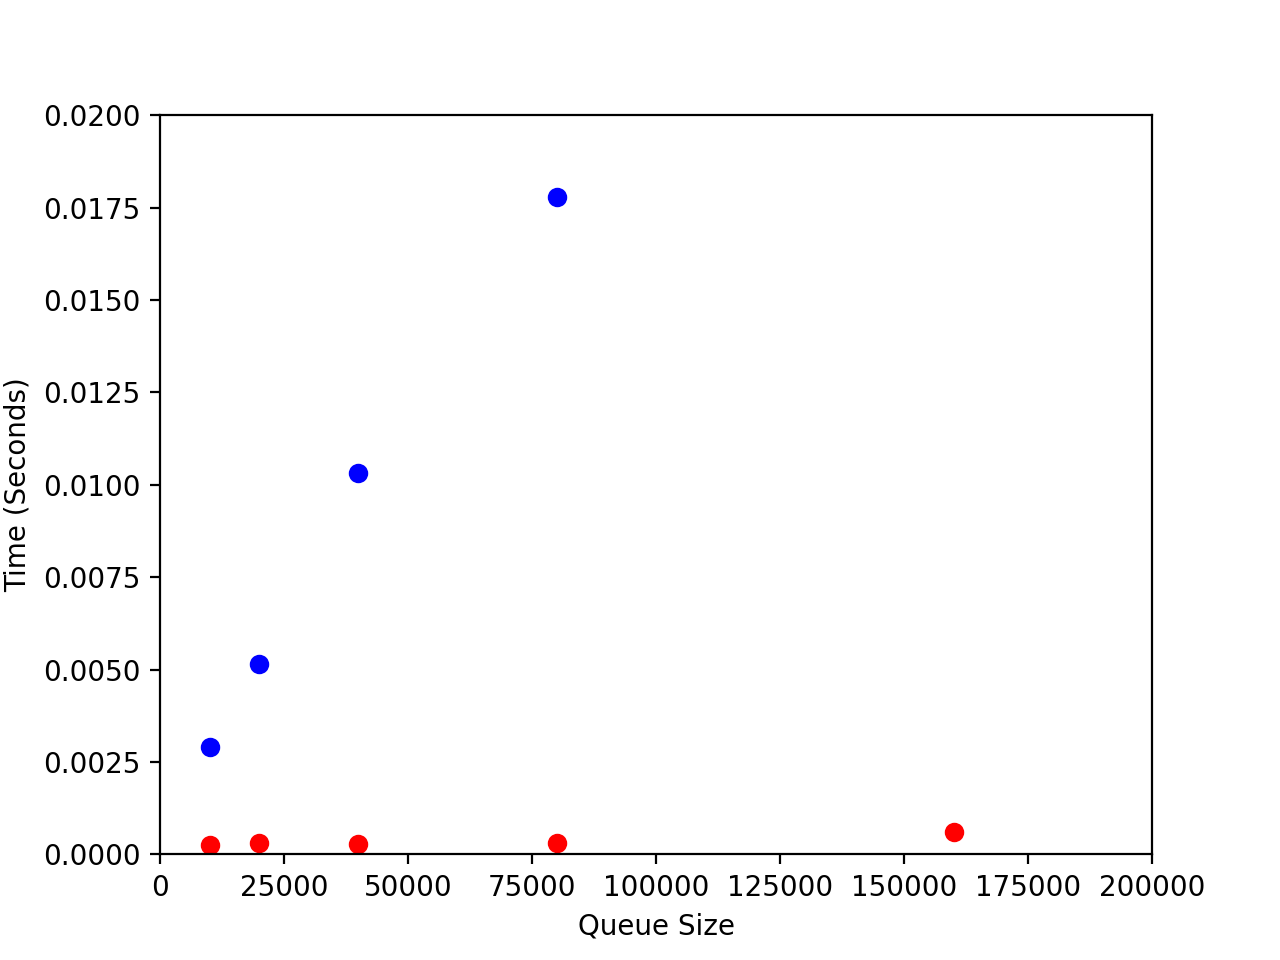
\includegraphics[width=0.8 \linewidth]{../../images/lab4_t4_q1_part3_solution.png}
    \end{center}

    \end{mdframed}

    \item If you still have time, explore! There’s lots of customization you can
    do with \textit{matplotlib} to make your graphs really pretty.
\end{enumerate}

\subsection*{Undo and redo}
\begin{itemize}
    \item

    \begin{lstlisting}[language=Python,caption={task\_4\_q1\_part\_3\_solution.py},captionpos=b]
    from mystack import Stack

    current_string = ''
    undo_stack = Stack()
    redo_stack = Stack()

    print('Please type one of the following commands:')
    print('REDO - redo undoed action')
    print('UNDO - show previously registered string')
    print('ADD - Add new string')
    print('EXIT - exit program')

    # 1. Prompt string
    while True:
        print('Current string: {}'.format(current_string))
        print(undo_stack._items)
        response = input('>>> ')

        # 2. If user types 'EXIT', then exit program
        if response == 'EXIT':
            break
        # 3. If user types 'UNDO',
        elif response == 'UNDO':
            #   3.1 If stack for undo is empty, return nothing
            if undo_stack.is_empty():
                continue

            #   3.2 If stack for undo not empty, then pop an item, push a copy to
            #   redo and display value to user
            redo_stack.push(current_string)
            undo_popped_val = undo_stack.pop()
            current_string = undo_popped_val

        # 4. If user types 'REDO'
        elif response == 'REDO':
            #   4.1 If stack for redo is empty, return nothing
            if redo_stack.is_empty():
                continue

            #   4.2 If stack for redo not empty, then pop an item, push a copy to
            #   undo and display value to user
            undo_stack.push(current_string)
            redo_popped_val = redo_stack.pop()
            current_string = redo_popped_val

        else:
            undo_stack.push(current_string)
            current_string = response
            redo_stack = Stack()
    \end{lstlisting}

    \bigskip

    When a user types new string after typing 'REDO', then the current list of stack items
    for redo should become clear.
\end{itemize}

\bigskip

\underline{\textbf{Notes:}}

\bigskip

\begin{itemize}
    \item 여보, 형모 공부하면서 노래 듣고 있었어요.
    \item \href{https://www.youtube.com/watch?v=Eh9JU_l7yN0}{요기}
    \item 형모 듣으면서 형모 평생 찾던 행복 찾게 해줘서 고마워요 생각하고 있었어요
    \item 당신 덕분에 형모 오늘 걸어요
    \item 여보, 태어나줘서 고마워요
    \item 여보 형모 여보 많이 사랑해
\end{itemize}

\end{document}
